Advances in processor efficiency along with the development of
energy-harvesting systems has created a new category of devices that require
neither a battery nor a tethered power
supply~\citep{prasad_comst_2014,lucia_snapl_2017,soyata_csm_2016}. These
devices operate using ambient energy, such as radio frequency
transmissions~\citep{rf_powered_computing_gollakota_2014},
light~\citep{margolies_infocom_2016,margolies_tosn_2016}, and
vibration~\citep{gorlatova_sigmetrics_2014}. Incorporating compute, storage,
sensing, and communication hardware~\citep{wisp5,moo,capybara}, such devices are a
promising technology for use in the Internet of Things~\citep{ku_cst_2016},
in-body~\citep{nadeau_naturebio_2017} and
on-body~\citep{bandodkar_electroanalysis_2015} medical systems, and
energy-harvesting nano-satellites~\citep{kicksat,capybara}.

Energy-harvesting devices create unique challenges because they operate {\em
intermittently} when energy is
available~\citep{hicks_isca_2017,lucia_snapl_2017}. An energy-harvesting device
buffers energy in a small storage capacitor~\citep{gorlatova_tmc_2013,gunduz_commag_2014} and operates when a
threshold amount of energy has accumulated. 
%
Harvestable energy sources are low-power (e.g., nW to $\mu$W) compared to a platform's operating
power level (hundreds of $\mu$W to mW). A device operates briefly until it depletes its buffered energy, after which, the device shuts
down and recharges to operate again later. As an example, recharge times may be
tens of seconds in radio frequency powered medical device~\cite[Fig.
3c]{nadeau_naturebio_2017}.  The recharge and discharge time --- which corresponds to the device's inactive and active time --- varies with the energy buffering capacitor's~\cite{capybara} and some devices fail and restart operating $\approx$10 to
$\approx$100 times per second~\citep{tan_infocom_2016,mementos,nvp}.

%\begin{figure}
%	\begin{subfigure}[t]{.35\linewidth}
%		\centering\large Figure
%		\caption{\centering WISP~\citep{wisp} against an RFID antenna}\label{fig:1a}
%	\end{subfigure}%
%	\begin{subfigure}[t]{.65\linewidth}
%		\centering\large Figure
%		\caption{\centering Program X~\citep{hicks_mibench2_2016} (split into X and Y tasks~\citep{chain}) at two distances}\label{fig:1b}
%    \end{subfigure}
%	\caption{Impact of an inadequate task sizing on the computation speed of a moving transiently-powered device.}\label{fig:1}
%\end{figure}

\begin{wrapfigure}{t!}{0.5\textwidth}
    \centering
    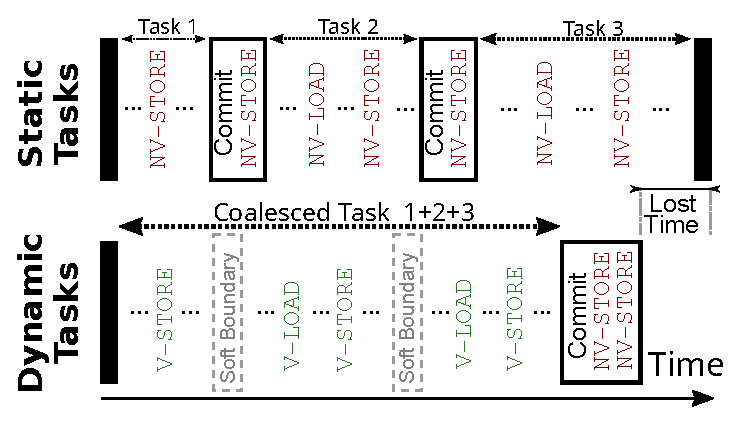
\includegraphics[width=0.5\textwidth]{figures/coalescing-is}
    \caption{\textbf{An execution of three
statically-defined tasks without (top) and with (bottom) dynamic
coalescing.} Task coalescing at runtime reduces time and energy overhead in
task-based intermittent programming models by performing fewer commits and
buffering updates to non-volatile (NV) variables in volatile (V) memory.}
    \label{fig:coalesce}
\end{wrapfigure}

\textbf{Data Consistency in Intermittent Computing.}  Software in an
energy-harvesting system operates according to the {\em intermittent execution
model}~\citep{dino,lucia_snapl_2017}, which corresponds to the
operation-failure-restart cycles of an energy-harvesting device. In an
intermittent software execution, an {\em operating period} proceeds for an
arbitrary duration (dictated by energy availability) before being interrupted
by a {\em failure period}. In a failure period, a device loses the volatile
state in its registers, stack, SRAM, and retains the state of any non-volatile
memory, such as FRAM or Flash. While capturing periodic
checkpoints~\citep{mementos,quickrecall} and sleep
scheduling~\citep{dewdrop,hibernus,hibernusplusplus} help preserve execution
progress, failures can leave non-volatile state incorrectly, partially updated,
and may leave checkpointed volatile state inconsistent with non-volatile state.
These inconsistencies cause intermittent executio to deviate from
continuously-powered behavior, often leading to an unrecoverable
application failure~\citep{dino,edb}. 

Prior work developed two main approaches to dealing with data inconsistency for
intermittently-powered devices: (i) \emph{software-based programming and
execution models}~\citep{dino,ratchet,chain,alpaca} and (ii)
\emph{hardware-based computer architecture
support}~\citep{hicks_isca_2017,idetic,nvp}.  Complex architectural changes are
expensive to design, verify, and manufacture.  New architectures are also
inapplicable to existing systems~\citep{hicks_isca_2017,nvp}. Software
approaches are simpler and applicable to existing devices today, but prior
software approaches have a number of limitations that are the focus of the work
in this paper.  A key limitation of prior software approaches that we address in this paper is the {\em inflexibility}
of a program statically decomposed into tasks. 

%\textcolor{red}{tictpl is not HW, is it? also it doesn't deal with inconsistency; this paragraph doesn't include Hibernus, so it should not include CPTL either.} 

% <<<<<<< HEAD
% \begin{figure}
% 	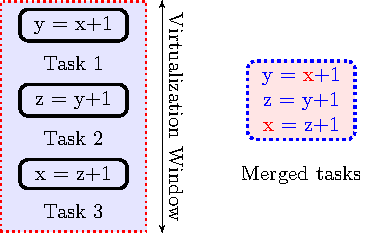
\includegraphics[width=.5\columnwidth]{figures/alpaca-war.pdf}
% 	\caption{\label{fig:virtualization}Adaptive task division at run-time might lead to write-after-read dependencies (variable \ttfamily{x}) that do not exist with static task division.\todo{Box with Task 1,2,3 must be the same size as merged task; Merged task must be named as Task 4; x must be marked in text as having WAR; "Task X" name should be next to the task box; "Window" - small letter}{Sinan}}
% \end{figure}
% =======

%Moved intel note to related work
\textbf{Task Decomposition of Intermittent Programs.} {\em
Task-based} programming and execution models require a
programmer~\citep{alpaca,chain} or a compiler~\cite{baghsorkhi_cgo_2018} to
statically decompose a program into a collection of {\em tasks}.  A task can
include arbitrary computation and these existing systems guarantee that each
tasks executes {\em atomically}, despite arbitrarily-timed power failures.  
%
The programmer explicitly expresses task-to-task control flow, or the compiler
converts existing program control-flow into task-to-task control flow to sequence 
the tasks that it defines.
%
Figure~\ref{fig:coalesce} (top) illustrates how a program's tasks execute and
shows how tasks can impose a run-time overhead. 
%
At each task transition, the system incurs an overhead to track and atomically
commit modifications to the non-volatile memory, to maintain consistency of
program state~\citep{chain,alpaca}.  
%
The more task transitions a program executes at run time, the more overhead.

A savvy programmer may thus create very large tasks in an attempt to
minimize overhead by minimizing the number of task transitions.  However, a
very large task may require more energy to complete than a device's fixed
hardware energy buffer can hold.  Such a large task fails to completely execute
assuming only buffered energy is available (i.e., assuming the worst case).
While some environments may have sufficient harvestable energy replenish the
capacitor during operation, enabling the task to complete, assuming cooperation
from the physical environment to avoid non-termination is a risky programming
proposition.  To eliminate this risk, existing systems require the programmer
or compiler to decompose a  program into small tasks, all of which complete
using only buffered energy.  These constraints on task sizing leave an
unsatisfying dilemma: large, efficient tasks that risk non-termination, or
small tasks that are guaranteed to complete, but incur a high task transition
and commit overhead.  In this work, we propose a third way, using a novel
technique called {\em dynamic task coalescing} that efficiently executes small
tasks, avoiding unnecessary overheads and avoiding the risk of non-termination.

%Brandon: I moved Cleancut to the related work section.  THere's too much in the intro already

%A key challenge is that the length of a software
%task's execution is \emph{limited by the fixed total amount of energy} that a
%device can buffer in hardware. A task's code is static, but the duration of its
%execution may be input-dependent and is difficult to predict. To illustrate
%this, we refer to Figure~\ref{fig:1} showing the execution time of two
%applications (the same application X, but divided into X and Y tasks as
%in~\citep{chain}) running on RFID antenna-powered Computational
%RFID~\citep{wisp,rf_powered_computing_gollakota_2014} at two device-to-antenna
%distances (near---stable energy supply/far---high energy intermittency). At
%short distance: execution will takes too long caused by runtime cost of
%marshalling excessively small tasks. At far distance: program \emph{might never
%execute} if task execution consumes more energy than the system can buffer.
%This calls for at-runtime adaptive task division of any transiently-powered
%application---namely \emph{task virtualization}.

\textbf{Task Coalescing.} In this work, we introduce a new system called \sys, which executes a task-based
intermittent program by dynamically coalescing its tasks.
\sys accepts any static decomposition (i.e., from the programmer or from a compiler) 
and coalesces its tasks at runtime. Two consecutive, coalesced tasks execute  
with no commit or task transition overhead between them, instead performing
task-end commit actions at the end second task only.
%
When there is sufficient energy to execute both tasks, two distinct, small
tasks are effectively executed as a single large task, preserving the atomicity
of both.  If power fails during a coalesced task, execution restarts from the
{\em first} of the coalesced tasks.  Figure~\ref{fig:coalesce} (bottom)
illustrates how dynamic coalescing changes the earlier execution and highlights
the change in memory model necessary to not break atomicity.

%Brandon: This is too detailed for the intro:
%Unfortunately, naively merging two atomic tasks might produce a non-atomic
%task, that may leave non-volatile memory inconsistent after a partial
%execution. A merge breaks atomicity when atomic merged tasks form a
%\emph{write-after-read (WAR)} dependency---for instance if two tasks
%\texttt{\{x=y+1\}; \{y=x;\}} are merged and if the power failure occurs after
%\texttt{x=y}, the value \texttt{x} will be increased twice when the merged task
%is restarted, that leads to an inconsistency.

%
%variables in non-volatile memory at \emph{run-time} that can
%break the atomicity of the \emph{virtual task}. Consider the
%example depicted in Fig.~\ref{fig:virtualization}: Tasks 1,
%2 and 3 being executed consecutively. All tasks in this
%example are atomic since they do not have WAR dependency on
%the persistent variables they are accessing, e.g. \emph{x}
%is only read and \emph{y} is only written within Task 1.
%Now, suppose three tasks have been virtualized into a single
%one at run-time, namely Task 4: since \emph{x} is now first
%\emph{read} and then \emph{written}, a WAR dependency on
%\emph{x} is introduced dynamically at
%run-time---unfortunately Task 4 is \emph{no more atomic}
%since its re-execution will not always produce the same
%results.
%
%Brandon: Sentence too long.
While a compiler can use static data privatization and commit instrumentation
(i.e., redo-logging) to eliminate statically identifiable, inter-task data
dependences~\citep{alpaca}, a \emph{dynamic} dependence between two coalesced
tasks requires dynamic privatization and commit actions. 
%
To ensure consistency and respect inter-task dependences, \sys uses a novel
approach to \emph{memory virtualization} that buffers non-volatile variable
updates in volatile memory during coalesced task execution, before committing
them to non-volatile memory at the dynamic task boundary.
%
%Therefore, we require a \emph{new execution
%model} that keeps each virtual task atomic by committing the
%modified persistent variables at the boundary defined
%dynamically at run-time---keeping the non-volatile memory
%unmodified upon a power-interrupt and preserving its
%consistency.

\textbf{Task Splitting}: A static task decomposition model assumes that each
single task can execute to completion.  If the hardware energy buffer provides
inadequate energy to execute each single task to completion, a program will not
terminate~\cite{cleancut}. To avoid non-termination under adversarial 
energy conditions, \sys uses a timer-based {\em partial task commit} mechanism.
Partial commit avoids non-termination by committing the intermediate state of a long-running
task that has repeatedly failed and restarted.  Partial commit violates
task atomicity, but preserves forward progress; if a programmer knows that
task atomicity is crucial to correctness, they can disable partial commit
instead risking non-termination.

%Task coalescing removes the burden from the programmer, because it accepts any
%task decomposition and improves it dynamically. To further reduce the
%programmer effort, we propose a compiler pass for \emph{automatic
%decomposition} of programs into (small) \emph{atomic} tasks. The compiler
%identifies non-volatile variables shared across tasks as tasks are created, and
%instruments reads and writes of those variables, using memory virtualization,
%to keep the data consistent in the presence of power loss.
%
%\textcolor{red}{Despite being limited to a subset of the C language, the
%automatic task decomposition allowed us to port several	applications to an
%intermittent platform with a moderate effort.}

\textbf{Contributions.} We develop \sys\footnote{To be released at
\url{http://anonymized.link}}: the first task coalescing system for task-based
programming models on intermittently-powered devices. The capabilities required
for effective coalescing mark our contributions:

\begin{itemize}
	\item \textcolor{red}{XXX} adaptive coalescing strategies for selecting boundaries to coalesce based on past execution behaviour;
	\item Software memory virtualisation for transiently-powered devices that preserves atomicity of coalesced tasks;
	\item Task splitting startegy that preserve forward progress and memory consistency;
\end{itemize}

%Existing programming and execution models may require more accesses to non-volatile memory (for multi-versioning)~\citep{dino,chain} or may preclude the use of volatile memory~\citep{ratchet}. Effective use of both volatile and non-volatile memory is important for \emph{efficiency}, because non-volatile memory has higher access energy and latency than SRAM~\citep{nvp}, and \emph{generality}, because devices often have much more FRAM than SRAM (e.g., 64 times more in~\citep{wolverine}). How to connect this trade-off with task virtualization remains an open question.

%\textbf{Research Question and Contributions:} Specifically, we ask (i) how to use software support to \emph{dynamically adapt} the effective size of a task, while respecting programmer-specified task atomicity, and (ii) how to minimize run time and energy consumption while \emph{automatically maintaining memory consistency} during execution?

%To address this question, we develop {\bf \sys}: a new programming and execution model efficiently executing tasks which avoids non-termination across a range of energy buffer sizes, without burdening the programmer\footnote{Code will be available via \href{http://anonymized.link}{http://anonymized.link}.}. To accomplish this, \sys introduces two new capabilities: 

%\begin{itemize}
%	\item {\bf Dynamic task coalescing:} \sys's task coalescing mechanism dynamically executes multiple tasks as a single task. A programmer or compiler can specify small tasks that will execute on a device with a small energy buffer. Coalescing tasks allows running the same tasks on a device with a larger energy buffer, avoiding run time overheads associated with ending one task and beginning another.
%	%
%	\item {\bf Volatile memory virtualization with transiently-powered device:} Colascing through task virtualization requires memory virtualization. \sys's uses SRAM as working memory, which \sys dynamically populates with pages of data from FRAM on demand, during a task's execution. When a task ends, \sys commits dirty pages to FRAM using DMA block copies, ensuring task atomicity and memory consistency. To the best of our knowledge this is the first time when memory virtualization has been demonstrated on a transient power budget.
%\end{itemize}

We evaluated \sys end-to-end on a real energy-harvesting device~\citep{wisp}
running existing benchmarks~\citep{chain,alpaca} and new programs. A comparison
to a state-of-the-art task-based system~\citep{chain,alpaca} showed that \sys
recovers performance on conservative task decompositions missed by systems with
static decomposition.
%
%and can flexibly target a variety of platforms without rewriting code.
%
%\todo{Provide concrete numeric results supporting this claim}{Amjad/Przemek}

%In this work we also address the problem of task construction burden imposed on the programmer. That is, we introduce \sys's compiler that transforms arbitrary C code into a graph of tasks that reflects the original program's control- and data-flow constraints. The compiler identifies data shared by multiple of the newly created tasks and instruments reads and writes of those data so that \sys's memory virtualization mechanism keeps those data consistent. While \sys's complier is still \emph{limited in scope}, e.g. is unable to handle instruction jumps, normalized loops and recursions, it already eliminates the labour-intensive process of writing tasks~\citep{chain,alpaca}, i.e., hours of programmer time.

%\sys's core contribution is the introduction of dynamic task coalescing mechanism. It allows the programmer or a compiler to intuitively decompose the program into small tasks that amortize fixed per-task overheads, yet present no risk of exceeding device energy capacity. As such a decomposition executes, \sys~{\em coalesces dynamically} consecutive tasks. Coalescing elides the commits of coalesced tasks by buffering multiple tasks' updates in an FRAM commit buffer. Periodically, as the span of the coalesced task grows, \sys ends coalescing and commits the state of the coalesced task. If a power failure interrupts a sequence of coalesced tasks, \sys adaptively reduces the number of tasks in that sequence that it will coalesce, committing sooner in future executions. Consequently, \sys's coalescing mechanism allows a program to execute efficiently across a range of energy buffer sizes, avoiding transition overheads in larger buffers, and ensuring progress in smaller buffers.

%We propose and explore two data swapping strategies for intermittently-powered systems based on FRAM/SRAM architecture. The first strategy is {\em demand paging}, which swaps the SRAM page with a new page from FRAM, buffering the swapped-out page until commit. The second strategy is {\em buffered direct access}, which directly reads and writes FRAM relying on dynamic double-buffering to ensure memory is consistent at commit.
